\let\negmedspace\undefined
\let\negthickspace\undefined
\documentclass[journal,12pt,twocolumn]{IEEEtran}

\usepackage{cite}
\usepackage{amsmath,amssymb,amsfonts,amsthm}
\usepackage{algorithmic}
\usepackage{graphicx}
\usepackage{textcomp}
\usepackage{xcolor}
\usepackage{txfonts}
\usepackage{listings}
\usepackage{enumitem}
\usepackage{mathtools}
\usepackage{gensymb}
\usepackage[breaklinks=true]{hyperref}
\usepackage{tkz-euclide} % loads  TikZ and tkz-base
\usepackage{listings}
\usepackage{circuitikz}
\usepackage{graphicx}

%\newcounter{MYtempeqncnt}
\DeclareMathOperator*{\Res}{Res}
%\renewcommand{\baselinestretch}{2}
\renewcommand\thesection{\arabic{section}}
\renewcommand\thesubsection{\thesection.\arabic{subsection}}
\renewcommand\thesubsubsection{\thesubsection.\arabic{subsubsection}}

\renewcommand\thesectiondis{\arabic{section}}
\renewcommand\thesubsectiondis{\thesectiondis.\arabic{subsection}}
\renewcommand\thesubsubsectiondis{\thesubsectiondis.\arabic{subsubsection}}

% correct bad hyphenation here
\hyphenation{op-tical net-works semi-conduc-tor}
\def\inputGnumericTable{}                                 %%

\lstset{
	frame=single,
	breaklines=true,
	columns=fullflexible
}



\newtheorem{theorem}{Theorem}[section]
\newtheorem{problem}{Problem}
\newtheorem{proposition}{Proposition}[section]
\newtheorem{lemma}{Lemma}[section]
\newtheorem{corollary}[theorem]{Corollary}
\newtheorem{example}{Example}[section]
\newtheorem{definition}[problem]{Definition}
\newcommand{\BEQA}{\begin{eqnarray}}
	\newcommand{\EEQA}{\end{eqnarray}}
\newcommand{\define}{\stackrel{\triangle}{=}}
\newcommand\figref{Fig.~\ref}
\newcommand\tabref{Table~\ref}
\bibliographystyle{IEEEtran}
%\bibliographystyle{ieeetr}


\providecommand{\mbf}{\mathbf}
\providecommand{\pr}[1]{\ensuremath{\Pr\left(#1\right)}}
\providecommand{\qfunc}[1]{\ensuremath{Q\left(#1\right)}}
\providecommand{\sbrak}[1]{\ensuremath{{}\left[#1\right]}}
\providecommand{\lsbrak}[1]{\ensuremath{{}\left[#1\right.}}
\providecommand{\rsbrak}[1]{\ensuremath{{}\left.#1\right]}}
\providecommand{\brak}[1]{\ensuremath{\left(#1\right)}}
\providecommand{\lbrak}[1]{\ensuremath{\left(#1\right.}}
\providecommand{\rbrak}[1]{\ensuremath{\left.#1\right)}}
\providecommand{\cbrak}[1]{\ensuremath{\left\{#1\right\}}}
\providecommand{\lcbrak}[1]{\ensuremath{\left\{#1\right.}}
\providecommand{\rcbrak}[1]{\ensuremath{\left.#1\right\}}}
\theoremstyle{remark}
\newtheorem{rem}{Remark}
\newcommand{\sgn}{\mathop{\mathrm{sgn}}}
\providecommand{\abs}[1]{\left\vert#1\right\vert}
\providecommand{\res}[1]{\Res\displaylimits_{#1}}
\providecommand{\norm}[1]{\left\lVert#1\right\rVert}
%\providecommand{\norm}[1]{\lVert#1\rVert}
\providecommand{\mtx}[1]{\mathbf{#1}}
\providecommand{\mean}[1]{E\left[ #1 \right]}
\providecommand{\fourier}{\overset{\mathcal{F}}{ \rightleftharpoons}}
%\providecommand{\hilbert}{\overset{\mathcal{H}}{ \rightleftharpoons}}
\providecommand{\system}{\overset{\mathcal{H}}{ \longleftrightarrow}}
%\newcommand{\solution}[2]{\textbf{Solution:}{#1}}
\newcommand{\solution}{\noindent \textbf{Solution: }}
\newcommand{\cosec}{\,\text{cosec}\,}
\providecommand{\dec}[2]{\ensuremath{\overset{#1}{\underset{#2}{\gtrless}}}}
\newcommand{\myvec}[1]{\ensuremath{\begin{pmatrix}#1\end{pmatrix}}}
\newcommand{\mydet}[1]{\ensuremath{\begin{vmatrix}#1\end{vmatrix}}}
\renewcommand{\abstractname}{Question}

\let\vec\mathbf

	
	\vspace{3cm}
	
	


\newcommand{\permcomb}[4][0mu]{{{}^{#3}\mkern#1#2_{#4}}}
\newcommand{\comb}[1][-1mu]{\permcomb[#1]{C}}

%\IEEEpeerreviewmaketitle

\newcommand \tab [1][1cm]{\hspace*{#1}}
%\newcommand{\Var}{$\sigma ^2$}
\usepackage{amssymb}
\usepackage{amsmath}
\title{
	
\title{NCERT Physics 12.7 Q6}
\author{EE23BTECH11061 - SWATHI DEEPIKA$^{*}$% <-this % stops a space
}


}
\begin{document}

\maketitle

\textbf{Question:} 
Obtain the resonance frequency of a series LCR circuit with $L = 2.0\, H$, $C = 32\, \mu F$, and $R = 10\, \Omega$. What is the Q-value of the circuit.\\

\begin{figure}[!h]
	\centering
	
\begin{circuitikz}
    % Define components with values
    \draw (0,0) to [L, l=$2.0\, H$] (2,0)  % Inductor L
    to [R, l=$10\, \Omega$] (4,0)  % Resistor R
    to [C, l=$32\, \mu\mathrm{F}$] (4,-2)  % Capacitor C
    -- (0,-2) to (0,0);  % Connect back to the starting point

    % Add labels
    \node at (1,0.3) {$+$};
    \node at (1,-2.3) {$-$};
\end{circuitikz}

	\caption{LCR Circuit}
	\label{fig:2}
\end{figure}
     
\textbf{Solution: }
In Figure~\figref{fig:2} the following information is provided:
 
 

 \begin{table}[h]
 	\centering
 	\resizebox{6 cm}{!}{
 		
    \begin{tabular}{|c|c|c|}
    \hline
     \textbf{Symbol} & \textbf{Value} &
     \textbf{Description}\\
    \hline
     $x(n)$ &  $(4n+1)u(n)$ & The nth term of the sequence\\[6pt]
    \hline 
     $x(17)$ &  $?$ & 17nth term \\[6pt]
    \hline
     $x(24)$ &  $?$ & 24th term\\[6pt]
    \hline
     
\end{tabular}

 	}
 	\vspace{6 pt}
 	\caption{Parameters}
 	\label{tab:my_label} 
 \end{table}
 
 The equivalent s domain of the circuit is :

\begin{figure}[!h]
 \centering
    \begin{circuitikz}
    \draw(0, 0) -- (1, 0);
    \draw(1, 0) to [L, l = $j\omega L$](2, 0);
    \draw(2, 0) -- (3, 0);
    \draw(3, 0) to [C, l = $\frac{1}{j\omega C}$](4, 0);
    \draw(4, 0) -- (5, 0);
    \draw(5, 0) to [R, l = $R$](6, 0);
    \draw(0, 0) -- (0, -2);
    \draw[->] (0, -1) node[left] {$I(s)$} -- (0, -1);
    \draw(6, 0) -- (7, 0);
    \draw(7, 0) -- (7, -2);
    \draw(0, -2) -- (3, -2);
    \draw(7, -2) -- (7, -2);
    \draw(3, -2) to [sV, l = $V(s)$](4, -2);
    \draw(4, -2) -- (7, -2);
\end{circuitikz}

    \caption{LCR Circuit in s-domain}
    
\end{figure}

\begin{align}
\frac{V(s)}{I(s)} = H(s)
\end{align}

\begin{align}
\frac{V(s)}{I(s)} = R + sL + \frac{1}{sC}\label{eq: 1} 
\end{align}

At resonance, 
\begin{align}
    Ls + \dfrac{1}{sC} &= 0\\
    \implies s &= j\dfrac{1}{\sqrt{LC}} \label{eq: 6}
\end{align}

\begin{equation}
    s = j\omega_0 \label{eq: 7}
\end{equation}
Comparing equations \eqref{eq: 6} and \eqref{eq: 7}, we get

\begin{equation}
    \omega_0 = \dfrac{1}{\sqrt{LC}}\label{eq: 8}
\end{equation}

\begin{align}
I_s(t) = I_0 \sin(\omega t + \phi)
\end{align}

\begin{align}
    \frac{di}{dt} & = I_0 \omega \cos(\omega t + \phi).
\end{align}

\begin{align}
    V_s & = L \frac{di}{dt} \\
    & = L I_0 \omega \cos(\omega t + \phi).
\end{align}


\begin{align}
    \cos(\theta) & = \frac{e^{j\theta} + e^{-j\theta}}{2}.
\end{align}

\begin{align}
    V_s & = L I_0 \omega \left(\frac{e^{j(\omega t + \phi)} + e^{-j(\omega t + \phi)}}{2}\right).
\end{align}

\begin{align}
    V_s & = j\omega L I_0 \sin(\omega t + \phi).
\end{align}
\begin{align}
    V_s & = j\omega L I_s.
\end{align}
\begin{align}
    V_s & = s L I_s.\label{eq: 10}
\end{align}

\begin{align}
    V_R & = I_s \cdot R\label{eq: 13}
\end{align}

From \eqref{eq: 10} and \eqref{eq: 13} , 
\begin{align}
    Q &= \left(\dfrac{V_L}{V_R}\right)_{\omega_0} = \dfrac{\lvert{sLI(s)}\rvert}{\lvert RI(s) \rvert}\\
    \implies Q &= \dfrac{1}{\sqrt{LC}}\dfrac{L}{R}\\
    \implies Q &= \dfrac{1}{R}\sqrt{\dfrac{L}{C}}\label{eq: 9}
\end{align}

\begin{align}
\frac{V(s)}{I(s)} = 10 + 2s + \frac{1}{32 \times 10^{-6}s}
\end{align}

\begin{align}
H(s) = 10 + 2s + \frac{1}{32 \times 10^{-6}s}
\end{align}


From, \eqref{eq: 8} :

\begin{align}
\omega_0 = \frac{1}{\sqrt{2 \, \text{H} \times 32 \, \mu\text{F}}} = 125 \, \text{rad/s}
\end{align}

The resonant frequency is 125 $rad/s$.\\

From, \eqref{eq: 9} :
\begin{align}
Q = \frac{1}{10}\sqrt{\frac{2}{32 \times 10^{-6}}} = \frac{1}{40 \times 10^{-3}} = 25
\end{align}

Therefore, the quality factor of the LCR circuit is 25.\\


\begin{align}
     H(s) &= R + sL + \dfrac{1}{sC}\\
     \implies H(j\omega) &= R + j\omega L + \dfrac{1}{j\omega C}\\
     \implies \lvert H(j\omega) \rvert &= \sqrt{R^2 + \left(\omega L - \dfrac{1}{\omega C}\right)^2}
\end{align}

\begin{figure}[!h]
    \centering
    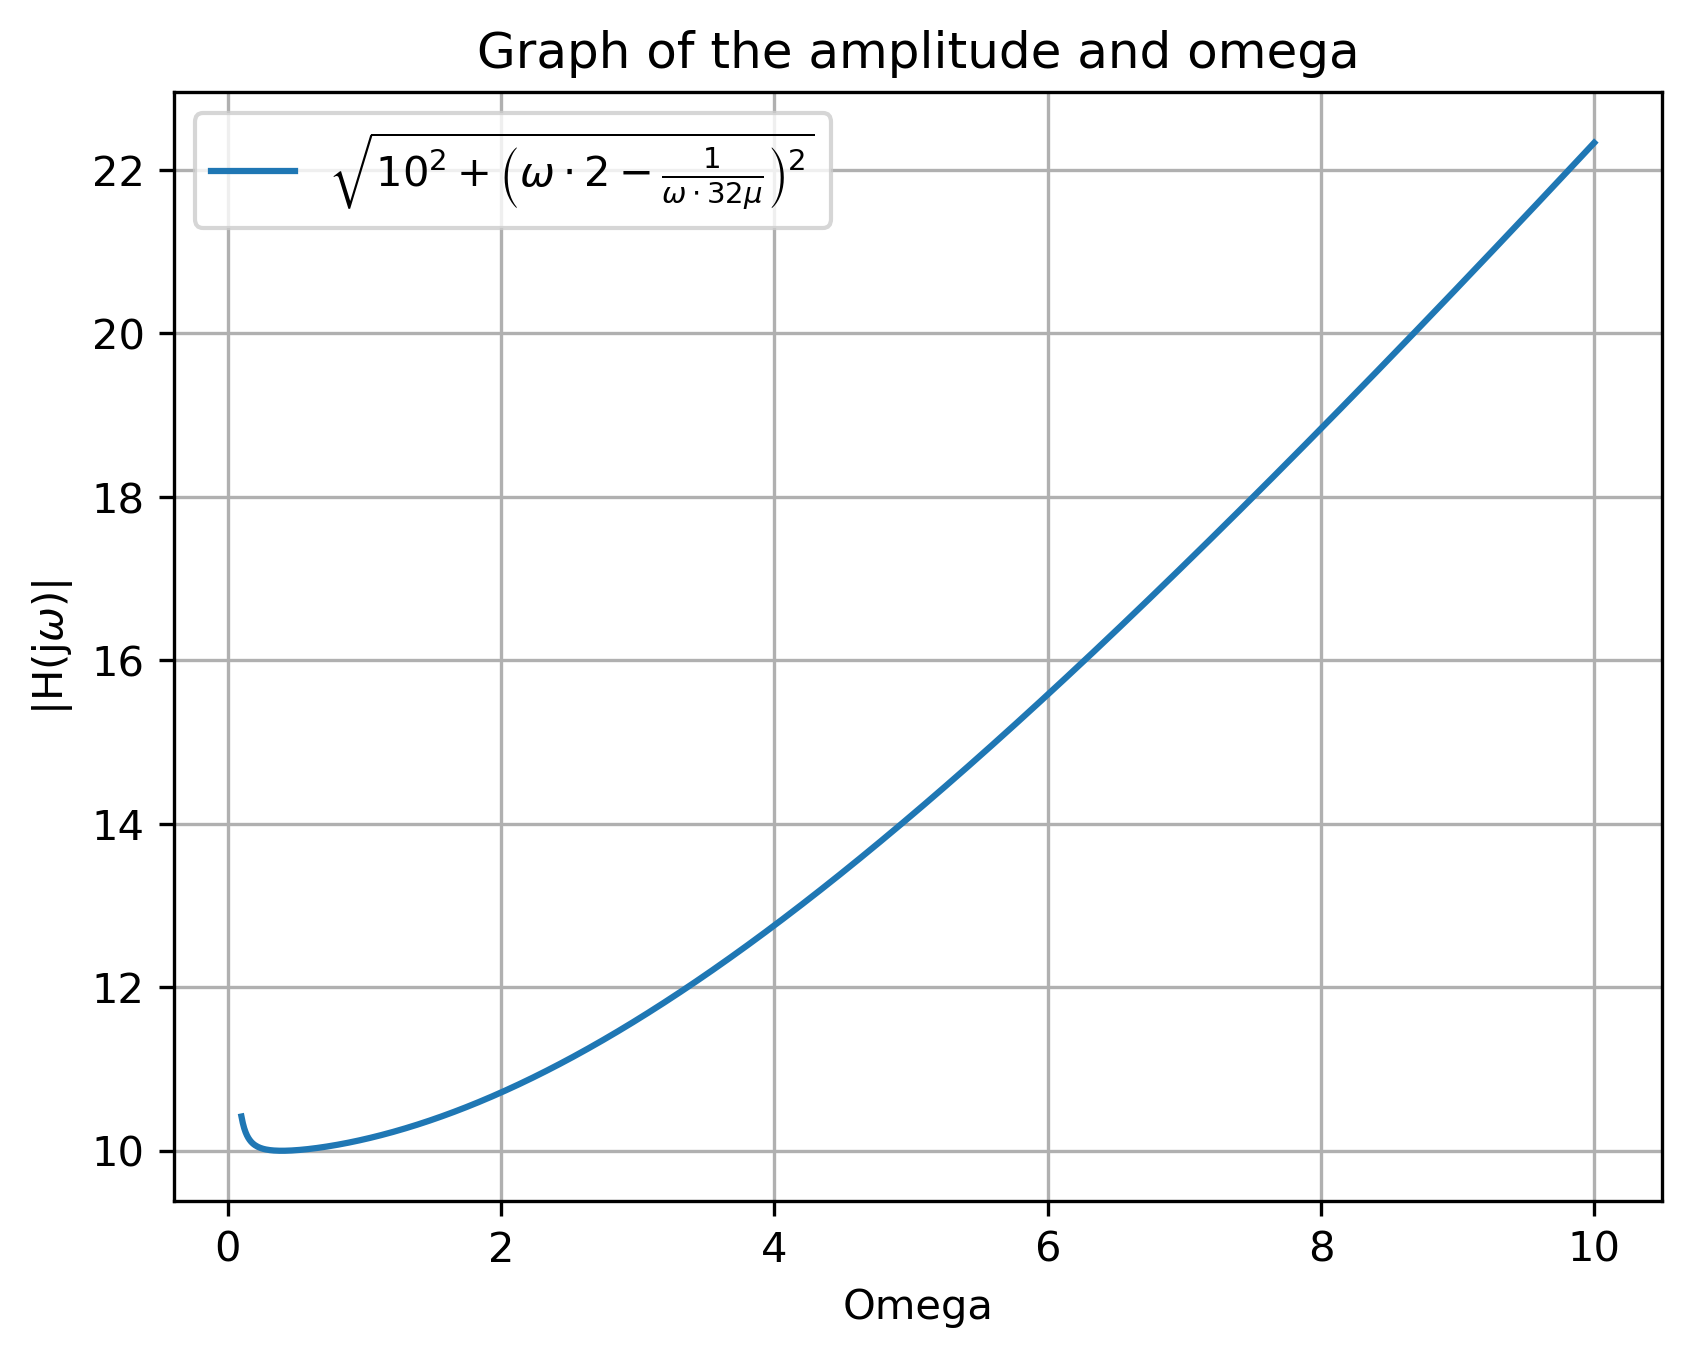
\includegraphics[width = \columnwidth]{figs/q_plot.png}
    \caption{Impedance vs $\omega$}
    \label{fig:h_plot}
\end{figure}


\end{document}



